\chapter{$\mathbf{T_{7}^{11}\sqcup T_{2}^{1}}$} \label{chap:special case}
To begin we construct $K_{14t+7}$ and $K_{14t+8}$ using joined copies of $K_{22}$, $K_{21}$, and $K_{14}$. Let $t$ be a positive integer. Now join $t-1$ copies of $K_{14}$ with each other and a lone copy of $K_{21}$. The resulting graph is $K_{14(t-1)+21} \cong K_{14t+7}$. Similarly, $K_{14t+8}$ can be constructed by joining $t-1$ copies of $K_{14}$ with each other and $1$ copy of $K_{22}$.

\begin{figure}[H]
    \begin{center}
      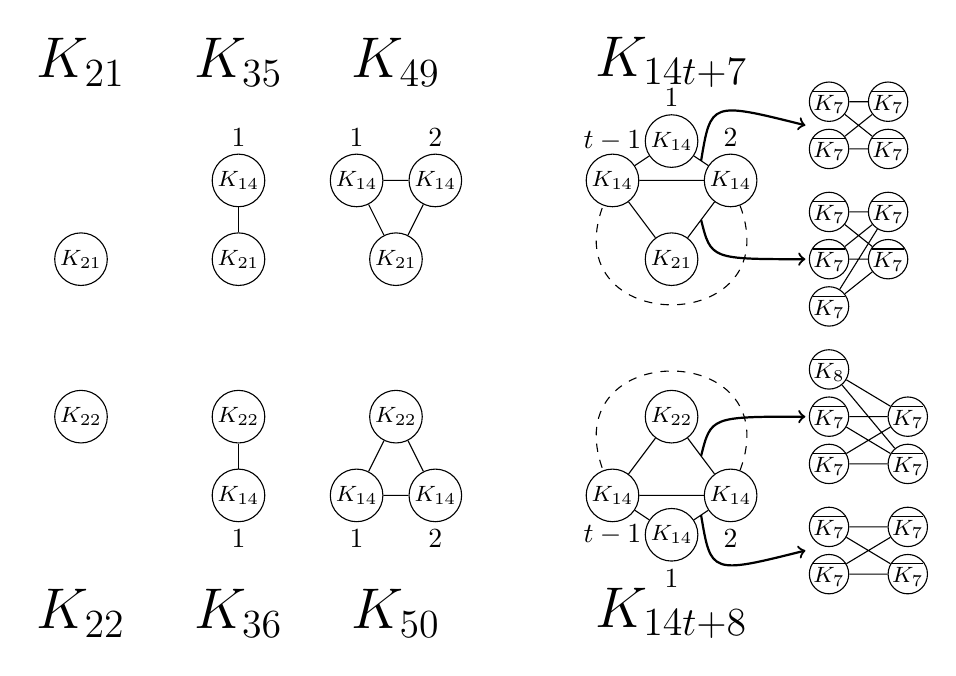
\begin{tikzpicture}[
        scale=1,
        smallnode/.style={draw,circle,inner sep=1pt,minimum size=6pt},
        bignode/.style={draw,circle,inner sep=0pt,minimum size=11pt}
      ]
        % Top header
        \node at (0,4.5)                   {\huge ${K_{21}}$};
        \node[smallnode] (K21) at (0,2)    {\footnotesize $K_{21}$};
  
        % K_35
        \begin{scope}[shift={(2,2)}]
          \node at (0,2.5)                {\huge${K_{35}}$};
          \node[smallnode] (A1) at (0,0)  {\footnotesize $K_{21}$};
          \node at (0,1.55)                {1};
          \node[smallnode] (B1) at (0,1)  {\footnotesize $K_{14}$};
          \draw (A1)--(B1);
        \end{scope}
  
        % K_49
        \begin{scope}[shift={(4,2)}]
          \node at (0,2.5)                {\huge${K_{49}}$};
          \node[smallnode] (A2) at (0,0)  {\footnotesize $K_{21}$};
          \node at (-.5,1.55)              {1};
          \node[smallnode] (B2) at (-.5,1){\footnotesize $K_{14}$};
          \node at (.5,1.55)               {2};
          \node[smallnode] (C2) at (.5,1) {\footnotesize $K_{14}$};
          \draw (A2)--(B2)--(C2)--(A2);
        \end{scope}
  
        % dots
        \node at (5.5,4.5) {\huge$\hdots$};
        \node at (5.5,3)   {\huge$\hdots$};
  
        % K_14t+7
        \begin{scope}[shift={(7.5,2)}]
          \node at (0,2.5)                     {\huge${K_{14t+7}}$};
          \node[smallnode] (A3) at (0,0)       {\footnotesize $K_{21}$};
          \node at (-.75,1.5)                 {$t-1$};
          \node[smallnode] (B3) at (-.75,1)    {\footnotesize $K_{14}$};
          \node at (0,2.05)                      {1};
          \node[smallnode] (C3) at (0,1.5)     {\footnotesize $K_{14}$};
          \node at (.75,1.55)                  {2};
          \node[smallnode] (D3) at (.75,1)     {\footnotesize $K_{14}$};
          \draw (A3)--(B3)--(C3)--(D3)--(A3)
                (B3)--(C3) (B3)--(D3) (C3)--(D3);
          \draw[dashed] (D3) .. controls (1.5,-1) and (-1.5,-1) .. (B3);
        \end{scope}
  
        % Last column top
        \begin{scope}[shift={(9.5,4)}]
          \node[bignode] (E1) at (0,0)    {\footnotesize$\overline{K_{7}}$};
          \node[bignode] (E2) at (0,-.6) {\footnotesize$\overline{K_{7}}$};
          \node[bignode] (F1) at (0.75,0)  {\footnotesize$\overline{K_{7}}$};
          \node[bignode] (F2) at (0.75,-.6){\footnotesize$\overline{K_{7}}$};
          \draw (E1)--(F1)--(E2) (E2)--(F2)--(E1);
        \end{scope}
  
        % Arrow 1 (unchanged)
        \path (C3) -- (D3) coordinate[midway] (M1);
        \path (E1) -- (E2) coordinate[midway] (M2);
        \path (M2)+(-.3,0) coordinate (M2);
        \draw[->,thick] (M1) .. controls (8,4) .. (M2);
  
        % Middle last column
        \begin{scope}[shift={(9.5,2.6)}]
          \node[bignode] (E3) at (0,0)    {\footnotesize$\overline{K_{7}}$};
          \node[bignode] (E4) at (0,-.6) {\footnotesize$\overline{K_{7}}$};
          \node[bignode] (E5) at (0,-1.2){\footnotesize$\overline{K_{7}}$};
          \node[bignode] (F3) at (0.75,0)  {\footnotesize$\overline{K_{7}}$};
          \node[bignode] (F4) at (0.75,-.6){\footnotesize$\overline{K_{7}}$};
          \draw (E3)--(F3)--(E4)
                (E4)--(F4)--(E3)
                (F3)--(E5)--(F4);
        \end{scope}
  
        % Arrow 2 (unchanged)
        \path (A3) -- (D3) coordinate[midway] (N1);
        \path (E4)+(-.3,0) coordinate (N2);
        \draw[->,thick] (N1) .. controls (8,2) .. (N2);
  
        % Mirrored last columns
        \begin{scope}[shift={(9.5,0.6)}]
          \node[bignode] (G1) at (0,0)   {\footnotesize$\overline{K_{8}}$};
          \node[bignode] (G2) at (0,-.6){\footnotesize$\overline{K_{7}}$};
          \node[bignode] (G3) at (0,-1.2){\footnotesize$\overline{K_{7}}$};
          \node[bignode] (H1) at (1,-.6){\footnotesize$\overline{K_{7}}$};
          \node[bignode] (H2) at (1,-1.2){\footnotesize$\overline{K_{7}}$};
          \draw (G1)--(H1)--(G2)
                (G2)--(H2)--(G1)
                (H1)--(G3)--(H2);
        \end{scope}
        \begin{scope}[shift={(9.5,-1.4)}]
          \node[bignode] (G4) at (0,0)   {\footnotesize$\overline{K_{7}}$};
          \node[bignode] (G5) at (0,-.6){\footnotesize$\overline{K_{7}}$};
          \node[bignode] (H3) at (1,0)  {\footnotesize$\overline{K_{7}}$};
          \node[bignode] (H4) at (1,-.6){\footnotesize$\overline{K_{7}}$};
          \draw (G4)--(H3)--(G5)
                (G5)--(H4)--(G4);
        \end{scope}
  
        % REFLECTED BELOW Y=0
        \node at (0,-2.5)                 {\huge${K_{22}}$};
        \node[smallnode] (K22) at (0,0)   {\footnotesize $K_{22}$};
  
        % Reflected K_36
        \begin{scope}[shift={(2,0)}]
          \node at (0,-2.5)                  {\huge${K_{36}}$};
          \node[smallnode] (R1) at (0,0)      {\footnotesize $K_{22}$};
          \node at (0,-1.55)                   {1};
          \node[smallnode] (R2) at (0,-1)     {\footnotesize $K_{14}$};
          \draw (R1)--(R2);
        \end{scope}
  
        % Reflected K_50
        \begin{scope}[shift={(4,0)}]
          \node at (0,-2.5)                  {\huge${K_{50}}$};
          \node[smallnode] (R3) at (0,0)      {\footnotesize $K_{22}$};
          \node at (-.5,-1.55)                 {1};
          \node[smallnode] (R4) at (-.5,-1)   {\footnotesize $K_{14}$};
          \node at (.5,-1.55)                  {2};
          \node[smallnode] (R5) at (.5,-1)    {\footnotesize $K_{14}$};
          \draw (R3)--(R4)--(R5)--(R3);
        \end{scope}
  
        % Reflected dots
        \node at (5.5,-2.5) {\huge$\hdots$};
        \node at (5.5,-1)   {\huge$\hdots$};
  
        % Reflected K_14t+8
        \begin{scope}[shift={(7.5,0)}]
          \node at (0,-2.5)                               {\huge${K_{14t+8}}$};
          \node[smallnode] (R6) at (0,0)                  {\footnotesize $K_{22}$};
          \node at (-.75,-1.5)                            {$t-1$};
          \node[smallnode] (R7) at (-.75,-1)              {\footnotesize $K_{14}$};
          \node at (0,-2.05)                                 {1};
          \node[smallnode] (R8) at (0,-1.5)               {\footnotesize $K_{14}$};
          \node at (.75,-1.55)                             {2};
          \node[smallnode] (R9) at (.75,-1)               {\footnotesize $K_{14}$};
          \draw (R6)--(R7)--(R8)--(R9)--(R6)
                (R7)--(R8) (R7)--(R9) (R8)--(R9);
          \draw[dashed] (R9) .. controls (1.5,1) and (-1.5,1) .. (R7);
        \end{scope}

        % Arrow 2 (mirrored)
        \path (R6) -- (R9) coordinate[midway] (N1);
        \path (G2)+(-.3,0) coordinate (N2);
        \draw[->,thick] (N1) .. controls (8,0) .. (N2);

        % Arrow 1 (unchanged)
        \path (R9) -- (R8) coordinate[midway] (M1);
        \path (G4) -- (G5) coordinate[midway] (M2);
        \path (M2)+(-.3,0) coordinate (M2);
        \draw[->,thick] (M1) .. controls (8,-2) .. (M2);
  
      \end{tikzpicture}
    \end{center}
    \caption{A different construction for $K_{14t+7}$ and $K_{14t+8}$.}
    \label{fig:newconstrK21K22}
  \end{figure}
Equivalently, We can view $K_{14t+7}$ as $K_{t}$ whose `vertices' are $K_{14}$ except one which is $K_{21}$, and whose edges are the join between them. We will refer to these `vertices' as nodes. Similarly, we can view $K_{14t+8}$ as $K_{t}$ whose nodes are $K_{14}$ except one which is $K_{22}$, and whose edges are the join between them. Notice in Figure \ref{fig:newconstrK21K22} that all edges in the $K_{t}$ constructions of these families are then the edges of $K_{14,14}$, $K_{21,14}$, and $K_{22,14}$.

We show that $\mathbf{T_{7}^{11}}\sqcup\mathbf{T_{2}^{1}}$ decomposes $K_{n}$ for $n\equiv7 \textrm{ or }8\pmod{14}$ where $n\geq 21$ by proving that $K_{22}$, $K_{21}$, $K_{14}$, $K_{22,14}$, $K_{21,14}$, and $K_{14,14}$ can each be decomposed by $\mathbf{T_{7}^{11}}\sqcup\mathbf{T_{2}^{1}}$ since these six graphs make up the nodes and edges of the $K_{t}$ representations of $K_{14t+7}$ and $K_{14t+8}$ where $t\geq 1$.

We begin with $K_{21}$ and $K_{22}$. The proof of the next theorem was obtained by manipulating a $K_{1,7}$-decomposition of $K_{21}$ by Cain in \cite{Cain1974}. We `plucked edges off' of every $7$-edge star in the decomposition, put them to the side, and then sent them to $6$-edge stars that they were vertex disjoint from. This gave us a $\mathbf{T_{7}^{11}}\sqcup\mathbf{T_{2}^{1}}$-decomposition of $K_{21}$, which can be found in Table \ref{tab:starpathK21}. Then, we just added three $6$-edge stars centered at $\infty$, and three distinct single edge paths from $\infty$ to the remaining three neighbors of $\infty$ in $K_{22}$ not covered in the stars. We once again put all the lone paths aside, and sent them to $6$-edge stars that they were vertex disjoint from them. This gave us a $\mathbf{T_{7}^{11}}\sqcup\mathbf{T_{2}^{1}}$-decomposition of $K_{22}$ which can be found in Table \ref{tab:starpathK22}.
\begin{thm}\label{thm:PCstarpath}
    $\mathbf{T_{7}^{11}}\sqcup\mathbf{T_{2}^{1}}$ decomposes $K_{21}$ and $K_{22}$.
\end{thm}

\begin{proof}
     Tables \ref{tab:starpathK21} and \ref{tab:starpathK22} give $\mathbf{T_{7}^{11}}\sqcup\mathbf{T_{2}^{1}}$-decompositions of $K_{21}$ and $K_{22}$, respectively.%The table will contain ad-hoc decompositions of $K_{21}$ and $K_{22}$. The construction for $K_{21}$ results from plucking edges off of Pauline Cain's $7$-star decomposition of $K_{21}$ and mixing them around, and The construction for $K_{22}$ results from adding three stars centered at $\infty$ and three lone paths beginning at $\infty$. Once again, edges are plucked off and mixed around to make this work.

\end{proof}
We did not need to develop anything formally to do this as we only performed this process once for the given $7$-edge star decomposition of $K_{21}$. Initially, we were interested in proving a stronger statement resulting from Cain's work, but found it difficult. Investigating implications of Cain's work \cite{Cain1974} from 1974 is something we are interested in for future work.

Next, we address $K_{22,14}$, $K_{21,14}$, and $K_{14,14}$. 
\newpage
\begin{thm} \label{thm:K_n,7}
    $\mathbf{T_{7}^{11}}\sqcup\mathbf{T_{2}^{1}}$ decomposes $K_{n,7}$ for all $n\geq 2$.
\end{thm}

\begin{proof}
    Consider $K_{n,7}$ where $n\geq 2$. Take the partite set of $n$ vertices to be $\ZZ_{n}$ and color them white. Similarly, take the partite set of $7$ vertices to be $K_{7}$ and color them black. Naturally, we refer to \textit{white-black} vertices $uv$ in $K_{n,7}$ via $(u,v)\in \ZZ_{n}\times\ZZ_{7}$ and vice versa. Finally, let $E_{i}=\{(i,0)\}\sqcup (\{i+1\}\times \{1,\hdots,6\})$ and $G_{i}\subset K_{n,7}$ be the subgraph induced by $E_{i}$ for each $i\in \ZZ_{n}$. Note that $G_{i}\cong \mathbf{T_{7}^{11}}\sqcup\mathbf{T_{2}^{1}}$ for all $i\in \ZZ_{n}$.

    \begin{figure}[H]
        \centering
        \documentclass{standalone}
\usepackage{amsmath,mathabx}
\usepackage{tikz}
\usetikzlibrary{positioning}
\begin{document}
    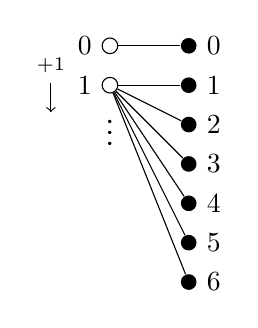
\begin{tikzpicture}[scale=0.5]
        %white
        \node[fill=white,draw =black, circle, inner sep=2pt, label=left:{\textcolor{black}{$0$}}] (w0) at (0,0) {};
        \node[fill=white,draw = black, circle, inner sep=2pt, label=left:{\textcolor{black}{$1$}}] (w1) at (0,-1) {};
        \node at (0,-2) {\large $\vdots$};

        %\node[draw=black, fill=white, circle, inner sep=1pt] (circ) at (-1.5,-0.5) {};
        \node (p1) at (-1.5,-0.5) {\scriptsize +1};
        \draw[->] ([yshift=0pt] p1.south) -- ++(0, -0.75);
        %black nodes
        \node[fill=black, circle, inner sep=2pt, label=right:{\textcolor{black}{$0$}}] (b0) at (2,0) {};
        \node[fill=black, circle, inner sep=2pt, label=right:{\textcolor{black}{$1$}}] (b1) at (2,-1) {};
        \node[fill=black, circle, inner sep=2pt, label=right:{\textcolor{black}{$2$}}] (b2) at (2,-2) {};
        \node[fill=black, circle, inner sep=2pt, label=right:{\textcolor{black}{$3$}}] (b3) at (2,-3) {};
        \node[fill=black, circle, inner sep=2pt, label=right:{\textcolor{black}{$4$}}] (b4) at (2,-4) {};
        \node[fill=black, circle, inner sep=2pt, label=right:{\textcolor{black}{$5$}}] (b5) at (2,-5) {};
        \node[fill=black, circle, inner sep=2pt, label=right:{\textcolor{black}{$6$}}] (b6) at (2,-6) {};
        \node at (0,-2) {\large $\vdots$};

        \draw[draw=black, shorten >=0pt, shorten <=0pt] (w0) -- (b0);
        \draw[draw=black, shorten >=0pt, shorten <=0pt] (w1) -- (b1);
        \draw[draw=black, shorten >=0pt, shorten <=0pt] (w1) -- (b2);
        \draw[draw=black, shorten >=0pt, shorten <=0pt] (w1) -- (b3);
        \draw[draw=black, shorten >=0pt, shorten <=0pt] (w1) -- (b4);
        \draw[draw=black, shorten >=0pt, shorten <=0pt] (w1) -- (b5);
        \draw[draw=black, shorten >=0pt, shorten <=0pt] (w1) -- (b6);
    \end{tikzpicture}
\end{document}
        \caption{$G_{0}$ in a generating presentation of the $\mathbf{T_{7}^{11}}\sqcup\mathbf{T_{2}^{1}}-$decomposition of $K_{n,7}$.}
        \label{fig:starpathbip}
    \end{figure}

    \noindent Notice that $E_{i}\cap E_{j}=\emptyset$ if $i\neq j$, so, by definition, all distinct $G_{i}$'s are pairwise edge disjoint. Lastly,
    $$\bigcup_{i\in \ZZ_{n}} E_{i}=[\bigcup_{i\in \ZZ_{n}} \{(i,0)\}]\sqcup [\bigcup_{i\in \ZZ_{n}} (\{i+1\}\times \{1,\hdots, 6\})]=[\ZZ_{n}\times \{0\}]\sqcup [\ZZ_{n}\times \{1,\hdots, 6\}]=\ZZ_{n}\times \ZZ_{7}.$$
    
    \noindent So, $G_{0}\cup \cdots \cup G_{n-1}=K_{n,7}$ and $\{G_{i}\mid i\in \ZZ_{n}\}$ is a $\mathbf{T_{7}^{11}}\sqcup\mathbf{T_{2}^{1}}-$decomposition of $K_{n,7}$. Furthermore, it is generated by developing the white vertices of $G_{0}$ by $1$.

\end{proof}

%old proof:

    %Take the partite set of $n$ nodes to be $\ZZ_{n}$ and color them white. Then, take the other partite set of $7$ nodes to be $\ZZ_{7}$ and color them black. Notice that $|E(K_{n,7})|=|\ZZ_{n}\oplus \ZZ_{7}|=7n$. So let us refer to edges of $K_{n,7}$ as elements of $\ZZ_{n}\oplus \ZZ_{7}$ and vice versa. Note that since $n\geq 2, (1,0)\neq (0,0)$.

    %Now, let $E_{i}= (i,0)+\{(0,0),(1,1),(1,2),\hdots,(1,6)\}$ for each $i\in \ZZ_{n}$ and $F_{i}$ be the subgraph induced by $E_{i}$. Since each $F_{i}$ contains a path $(i,0)$ which is vertex disjoint from the star centered at the white $i+1$, it must be isomorphic to $\mathbf{T_{7}^{11}}\sqcup\mathbf{T_{2}^{1}}$.

    %note to self: originally I thought of E_i's as (i,0) + (\{(0,0)\}\cup [(1,0)+[\langle (0,1)\rangle\setminus \{(0,0)\}]])

    %the union expression at the end is messy. However, the point of using groups here is basically that when we use generator notation we can swallow things up to get simpler things in terms of generators and it works out nicely here.
    
    %\noindent Suppose that there exist distinct $i,j\in \ZZ_{n}$ such that $E_{i}\cap E_{j}\neq \emptyset$. But then we have that $(i,0)=(j,0)$ or $(i+1,a)=(j+1,b)$ for some $a,b\in \ZZ_{7}$, which is impossible. So all distinct $E_{i}$'s are pairwise disjoint, and therefore all distinct $F_{i}$'s are pairwise edge-disjoint. Lastly, $\bigcup_{i\in \ZZ_{n}} E_{i}=\langle (1,0)\rangle + [\{(0,0)\}\cup [(1,0)+\langle (0,1)\rangle] \setminus \{(1,0)\}]=\langle (1,0)\rangle + \langle (0,1)\rangle = \langle (1,0),(0,1)\rangle = \ZZ_{n}\oplus \ZZ_{7}$. Therefore, $\bigcup_{i\in \ZZ_{n}} F_{i} = K_{n,7}$. \\

\begin{corollary}\label{cor:starpathbi}
    $\mathbf{T_{7}^{11}}\sqcup\mathbf{T_{2}^{1}}$ decomposes $K_{22,14}$, $K_{21,14},\text{ and }K_{14,14}$.
\end{corollary}

\begin{proof}
    $\mathbf{T_{7}^{11}}\sqcup\mathbf{T_{2}^{1}}$ decomposes $K_{7,7}$ and $K_{8,7}$ by Theorem \ref{thm:K_n,7}. $K_{14,14}$ can be expressed as the edge-disjoint union of four copies of $K_{7,7}$; $K_{21,14}$ can be expressed as the edge-disjoint union of six copies of $K_{7,7}$; and $K_{22,14}$ can be expressed as the edge-disjoint union of two copies of $K_{8,7}$ and four copies of $K_{7,7}$. Therefore, $\mathbf{T_{7}^{11}}\sqcup\mathbf{T_{2}^{1}}$ decomposes them all.

\end{proof}
Recall that we proved that $K_{14}$ and $K_{15}$ are $\mathbf{T_{7}^{11}}\sqcup\mathbf{T_{2}^{1}}$-decomposable in Chapter \ref{chap:0,1(mod 14)}. So, we are now ready to put everything together to state the main theorem of this chapter, completing the main result of this thesis.
\begin{thm}
$\mathbf{T_{7}^{11}}\sqcup\mathbf{T_{2}^{1}}$ decomposes $K_{14t+7}$ and $K_{14t+8}$ where $t$ is a positive integer. 
\end{thm}
\begin{proof}
We have that $\mathbf{T_{7}^{11}}\sqcup\mathbf{T_{2}^{1}}$ decomposes $K_{14}$ by Theorem \ref{thm:sigma plus minus}; $K_{22,14}$, $K_{21,14},\text{ and }K_{14,14}$ by Corollary \ref{cor:starpathbi}; and lastly $K_{22},K_{21}$ by Theorem \ref{thm:PCstarpath}.
\newline\newline
Therefore, $\mathbf{T_{7}^{11}}\sqcup\mathbf{T_{2}^{1}}$ decomposes the join of $(t-1)$ copies of $K_{14}$ with each other and $1$ copy of $K_{21}$, which is isomorphic to $K_{14t+7}$. Similarly, $\mathbf{T_{7}^{11}}\sqcup\mathbf{T_{2}^{1}}$ decomposes the join of $(t-1)$ copies of $K_{14}$ with each other and $1$ copy of $K_{22}$, which is isomorphic to $K_{14t+8}$.

\end{proof}

We have now solved the spectrum problem for every forest on seven edges. 